\section{Los Componentes de la aplicación}
El directorio \texttt{components} contiene todos los componentes reutilizables que forman la base de la interfaz de usuario de la aplicación. Estos componentes están organizados en subdirectorios según su funcionalidad y uso específico dentro de la aplicación , la cual esta estructurado de la siguiente forma .

\paragraph{Estrucutra de la carpeta components}
\begin{itemize}
\item \textbf{components/icons}: Este subdirectorio almacena todos los íconos utilizados en la aplicación, organizados por categorías como certificaciones, pilares de la empresa y redes sociales. Incluye también el logo principal de la aplicación.
\item \textbf{components/pages}: Este subdirectorio agrupa los componentes específicos de las diferentes páginas de la aplicación. Incluye componentes para páginas de cursos, la página principal y elementos globales como el encabezado y el pie de página.
\item \textbf{components/providers}: Este subdirectorio contiene componentes proveedores que gestionan aspectos globales de la aplicación, como la configuración del tema.
\item \textbf{components/ui}: Este subdirectorio contiene componentes reutilizables de la interfaz de usuario, tales como botones, tarjetas, carruseles y menús desplegables. Estos componentes son esenciales para construir la interfaz gráfica de la aplicación.
\end{itemize}

\subsection{Components/icons}
Este subdirectorio almacena todos los íconos utilizados en la aplicación, organizados por categorías. Incluye íconos para certificaciones, pilares de la empresa y redes sociales, así como el logo principal de la aplicación.

\subsubsection{components/iconscertifications}
Esta categoría contiene íconos relacionados con certificaciones específicas de la aplicación.
\begin{itemize}
    \item \textbf{Icon1.tsx}: Ícono para certificación tipo 1.
    \item \textbf{Icon2.tsx}: Ícono para certificación tipo 2.
    \item \textbf{Icon3.tsx}: Ícono para certificación tipo 3.
\end{itemize}

\subsubsection{components/iconspillars}
Esta categoría contiene íconos que representan los pilares fundamentales de la empresa.
\begin{itemize}
    \item \textbf{Icon1.tsx}: Ícono para pilar 1.
    \item \textbf{Icon2.tsx}: Ícono para pilar 2.
    \item \textbf{Icon3.tsx}: Ícono para pilar 3.
\end{itemize}

\subsubsection{components/iconssocial}
Esta categoría contiene íconos de las redes sociales utilizadas en la aplicación.
\begin{itemize}
    \item \textbf{FacebookLogo.tsx}: Ícono para Facebook.
    \item \textbf{InstagramLogo.tsx}: Ícono para Instagram.
    \item \textbf{TiktokLogo.tsx}: Ícono para TikTok.
    \item \textbf{TwitterLogo.tsx}: Ícono para Twitter.
\end{itemize}

\subsubsection{Logo.tsx}
Este componente es el logo principal de la aplicación.


\subsection{Components/providers}
Este subdirectorio contiene componentes que proporcionan contexto y servicios globales a la aplicación. Estos componentes están diseñados para gestionar aspectos globales y compartir datos entre diferentes partes de la aplicación.

\begin{itemize}
    \item \textbf{ThemeProvider.tsx}: Este componente utiliza el \texttt{NextThemesProvider} de la biblioteca \texttt{next-themes} para manejar el tema de la aplicación. Permite la aplicación de un tema predeterminado, la adaptación al sistema del usuario y la desactivación de transiciones en el cambio de tema. El componente envuelve a los hijos en el proveedor de temas, facilitando el control del tema en toda la aplicación.
\end{itemize}

\begin{minted}{typescript}
  import { ThemeProvider as NextThemesProvider } from 'next-themes';

  export function ThemeProvider({ children }: { children: React.ReactNode }) {
    return (
      <NextThemesProvider
        attribute="class"
        defaultTheme="system"
        enableSystem
        disableTransitionOnChange
      >
        {children}
      </NextThemesProvider>
    );
  }
\end{minted}

\subsection{Components/ui}
Este subdirectorio contiene componentes reutilizables de la interfaz de usuario que son fundamentales para construir la apariencia y funcionalidad de la aplicación.

\begin{itemize}
    \item \textbf{button.tsx}: Define un componente de botón reutilizable con variantes estilísticas (por ejemplo, default, destructive, outline, secondary, ghost, link) y tamaños (default, sm, lg, icon). Utiliza la librería class-variance-authority para manejar variantes de estilos y la biblioteca @radix-ui/react-slot para permitir el uso de componentes personalizados como hijos.
    \item \textbf{card.tsx}: Contiene un conjunto de componentes relacionados con la presentación de tarjetas. Card es el contenedor principal, mientras que CardHeader, CardTitle, CardDescription, CardContent y CardFooter estructuran diferentes partes de la tarjeta para organizar el contenido de forma clara y estilizada.
    \item \textbf{carousel.tsx}: Implementa un carrusel utilizando embla-carousel-react. El componente Carousel maneja la lógica del carrusel, incluyendo la navegación y la gestión del estado de desplazamiento. CarouselContent, CarouselItem, CarouselPrevious, y CarouselNext son subcomponentes para el contenido del carrusel, los ítems individuales y los botones de navegación, respectivamente. Utiliza el contexto de React para manejar el estado y las acciones del carrusel.
    \item \textbf{dropdown-menu.tsx}: Proporciona un conjunto de componentes para menús desplegables utilizando @radix-ui/react-dropdown-menu. Incluye DropdownMenu, DropdownMenuTrigger, DropdownMenuContent, DropdownMenuItem, y otros para construir menús complejos con soporte para submenús, casillas de verificación, y opciones de radio. Estiliza estos componentes para una apariencia consistente.
    \item \textbf{input.tsx}: Define un componente de entrada de datos estilizado. Permite la personalización del tipo de entrada y aplica estilos consistentes para el tamaño, el borde y los estados de enfoque o desactivado.
    \item \textbf{label.tsx}: Implementa un componente de etiqueta utilizando @radix-ui/react-label, estilizado con la librería class-variance-authority. Este componente se utiliza para asociar texto descriptivo con campos de formulario o elementos interactivos, con soporte para personalización de estilos.
    \item \textbf{sheet.tsx}: Define un componente de hoja modal utilizando @radix-ui/react-dialog. Incluye Sheet, SheetTrigger, SheetClose, SheetPortal, y SheetContent para manejar la presentación de un panel modal deslizante con varios efectos de entrada/salida. SheetHeader, SheetFooter, SheetTitle, y SheetDescription estructuran el contenido dentro del modal.
    \item \textbf{ThemeToggle.tsx}: Implementa un componente para alternar entre temas claros y oscuros en la aplicación. Utiliza la biblioteca next-themes para gestionar el tema actual y permite a los usuarios cambiar entre los temas utilizando botones con iconos de sol y luna.
\end{itemize}

\subsection{Components/pages} 
Los componentes que definen y estructuran el contenido específico de las diferentes páginas y secciones de la aplicación. Cada subdirectorio dentro de components/pages se dedica a una sección particular de la aplicación, como cursos, páginas de inicio o elementos globales. Los componentes en esta carpeta están diseñados para representar y organizar el contenido y la funcionalidad de cada página de manera modular y reutilizable, facilitando así el mantenimiento y la expansión de la interfaz de usuario de la aplicación.

\begin{itemize}
    \item \textbf{components/pages/home/} 
    \item \textbf{src/components/pages/global}
    \item \textbf{src/components/pages/courses}
    \item \textbf{src/components/pages/course}
\end{itemize}


\subsection{Componentes de components/pages/home/}
Se encuentran los componentes específicos para la página de inicio de la aplicación. Esta carpeta contiene componentes diseñados para presentar secciones clave en la página principal, como los pilares de la plataforma y el título principal.
    
  \begin{itemize}
    \item \texttt{Pillars.tsx}:
    \begin{itemize}
      \item Define una sección que presenta los pilares o fundamentos de la aplicación. 
      \item Utiliza un conjunto de iconos y etiquetas para ilustrar los conceptos clave.
      \item Los iconos se importan de la carpeta de iconos y se asocian con etiquetas descriptivas como Aprende, Crea, y Comparte.
      \item Cada pilar se representa dentro de un contenedor estilizado con una imagen del icono y un botón para la acción.
      \begin{minted}{typescript}
import Icon1 from '@/components/icons/pillars/Icon1';
import Icon2 from '@/components/icons/pillars/Icon2';
import Icon3 from '@/components/icons/pillars/Icon3';
import { Button } from '@/components/ui/button';
const UTILITIES = [
  {
    Icon: Icon1,
    label: 'Aorende',
  },
  {
    Icon: Icon2,
    label: 'Crea',
  },
  {
    Icon: Icon3,
    label: 'Comparte',
  },
];
export default function Pillars() {
  return (
    <section className="w-full max-w-6xl flex flex-col items-center justify-start gap-10 px-6 my-40">
      <h1 className="text-4xl font-bold text-center">Nuestros pilares</h1>
      <div className="flex gap-10 justify-around items-center flex-wrap w-full max-w-4xl">
        {UTILITIES.map(({ Icon, label }) => (
          <div
            key={crypto.randomUUID()}
            className="bg-card rounded-md py-6 px-14 flex flex-col items-center justify-center gap-4 shadow-md"
          >
            <Icon className="w-28 h-28 m-4" />
            <span className="text-2xl font-semibold">{label}</span>
            <Button variant="secondary" size="icon" className="mt-4">
              -&gt;
            </Button>
          </div>
        ))}
      </div>
    </section>
  );
}
      \end{minted}
    \end{itemize}
    \item \texttt{Title.tsx}:
    \begin{itemize}
      \item Presenta el título principal de la página de inicio.
      \item Incluye un encabezado que destaca el objetivo principal de la plataforma y un subtítulo que refuerza el mensaje central.
      \item Ofrece botones para acciones adicionales como "Ver más" y "Comienza ahora".
      \item Está diseñado para captar la atención del usuario y proporcionar información introductoria sobre la plataforma.
      \begin{minted}{typescript}
import { Button } from '@/components/ui/button';
export default function Title() {
  return (
    <section className="w-full max-w-6xl flex flex-col items-center justify-center gap-8 my-40">
      <h1 className="w-full flex flex-col items-center justify-center font-bold">
        <span className="text-5xl text-center">Aprende a programar y desarrollar</span>
        <span className="text-6xl text-primary text-center">con Learning</span>
      </h1>
      <p className="w-full max-w-sm text-center">
        la plataforma que te ayuda a mejorar tus habilidades en programación.
      </p>
      <div className="flex items-center gap-4 text-lg">
        <Button variant="secondary" size="lg">
          Ver mas →
        </Button>
        <Button size="lg">
          Comienza ahora
        </Button>
      </div>
    </section>
  );
}
      \end{minted}
    \end{itemize}
  \end{itemize}

\subsection{Componentes de components/pages/global/}
Contiene componentes que proporcionan funcionalidad y estructura global para la aplicación. Estos componentes incluyen elementos comunes y fundamentales, como encabezados, pies de página, y funciones de autenticación y perfil de usuario.
\begin{itemize}
  \item \texttt{Access.tsx}:
  \begin{itemize}
      \item Controla el acceso a la aplicación mostrando el componente de inicio de sesión (\texttt{Login}) si el usuario no está autenticado. Si el usuario está autenticado, muestra el componente de perfil (\texttt{Profile}) con la información del usuario.
      \item Usa la función \texttt{getServerSession} para verificar la sesión del usuario y renderiza el componente correspondiente basado en el estado de autenticación
      \begin{minted}{typescript}
import { authOptions } from '@/app/api/auth/[...nextauth]/authOptions';
import { getServerSession } from 'next-auth';
import Login from './Login';
import Profile from './Profile';
export default async function Access() {
  const session = await getServerSession(authOptions);
  if (!session) {
    return (
      <Login />
    );
  }
  return (
    <Profile
      name={session.user?.name || ''}
      email={session.user?.email || ''}
      image={session.user?.image || ''}
    />
  );
}
      \end{minted}
  \end{itemize}
  
  \item \texttt{BrandTitle.tsx}:
  \begin{itemize}
      \item Muestra el nombre de la marca acompañado de un logotipo. Es un componente simple que define el estilo del título de la aplicación.
      \item Utiliza el componente \texttt{Logo} para incluir un ícono y estiliza el texto de la marca.
      \begin{minted}{typescript}
import Logo from '@/components/icons/Log
export default function BrandTitle() {
  return (
    <div className="text-primary text-4xl font-bold flex gap-1">
      <Logo className="w-10 h-10" />
      <span>
        earning
      </span>
    </div>
  );
}
      \end{minted}
  \end{itemize}
  
  \item \texttt{Footer.tsx}:
  \begin{itemize}
    \item Se utilizan componentes íconos específicos para cada red social, importados desde rutas designadas.
    \item Cada ícono está vinculado a la página de la red social correspondiente mediante un enlace (\texttt{href}).
    \item Se incluye un componente \texttt{BrandTitle} que muestra el nombre de la marca.
    \begin{minted}{typescript}
import FacebookLogo from '@/components/icons/social/FacebookLogo';
import InstagramLogo from '@/components/icons/social/InstagramLogo';
import TwitterLogo from '@/components/icons/social/TwitterLogo';
import TiktokLogo from '@/components/icons/social/TiktokLogo';
import BrandTitle from './BrandTitle
const SOCIALS = [
  {
    Icon: FacebookLogo,
    href: 'https://www.facebook.com/learning',
    label: 'Facebook',
  },
  {
    Icon: InstagramLogo,
    href: 'https://www.instagram.com/learning',
    label: 'Instagram',
  },
  {
    Icon: TwitterLogo,
    href: 'https://www.twitter.com/learning',
    label: 'Twitter',
  },
  {
    Icon: TiktokLogo,
    href: 'https://www.tiktok.com/@learning',
    label: 'TikTok',
  },
];
export default function Footer() {
  return (
    <footer className="w-full border-t border-foreground/10 px-6 flex justify-between items-start py-6">
      <div className="flex flex-col gap-4">
        <BrandTitle />
        <span>
          © 2024 Learning. Todos los derechos reservados.
        </span>
      </div>
      <ul className="flex gap-6 items-center justify-center">
        {
          SOCIALS.map(({ Icon, href, label }) => (
            <li key={label}>
              <a href={href}>
                <Icon className="w-10 h-auto" />
                <span className="sr-only">{label}</span>
              </a>
            </li>
          ))
        }
      </ul>
    </footer>
  );
}
    \end{minted}
  \end{itemize}
  
  \item \texttt{Header.tsx}:
  \begin{itemize}
      \item Define la cabecera de la aplicación, incluyendo el logotipo, enlaces de navegación y componentes para el acceso de usuario y el cambio de tema.
      \item Incluye un logotipo y enlaces de navegación que se renderizan en una barra superior, y utiliza los componentes \texttt{Access} y \texttt{ThemeToggle} para funcionalidades adicionales.
      \begin{minted}{typescript}
import Logo from '@/components/icons/Logo';
import { ThemeToggle } from '@/components/ui/ThemeToggle';
import Link from 'next/link';
import Access from './Acces
export function Header() {
  const LINKS = [
    {
      label: 'Home',
      path: '/',
    },
    {
      label: 'Cursos',
      path: '/cursos',
    },
    {
      label: 'Planes',
      path: '/planes',
    },
  ];
  return (
    <header className="w-full px-6 flex justify-center items-center sticky top-0 backdrop-blur-md bg-neutral-100/40 dark:bg-slate-800/40 z-50">
      <div className="w-full max-w-6xl py-4 flex justify-between">
        <Link href="/" className="flex items-center gap-1 text-3xl font-bold text-primary">
          <Logo className="w-10 h-10" />
          <span>
            earning
          </span>
        </Li
        <nav className="flex gap-6 items-center">
          {
            LINKS.map(({ label, path }) => (
              <Link key={label} href={path} className="hover:underline">
                {label}
              </Link>
            ))
          }
          <Access />
          <ThemeToggle />
        </nav>
      </div>
    </header>
  );
}
      \end{minted}
  \end{itemize}
  
  \item \texttt{Login.tsx}:
  \begin{itemize}
    \item Proporciona un modal para el inicio de sesión de usuario. Permite el acceso mediante Google, Github o con correo electrónico y contraseña.
    \item Utiliza el componente \texttt{Sheet} para crear el modal, y dentro del modal incluye botones para iniciar sesión con diferentes métodos y un formulario para credenciales.
    \begin{minted}{typescript}
'use client';

import { Button } from '@/components/ui/button';
import { Input } from '@/components/ui/input';
import { Label } from '@/components/ui/label';
import {
  Sheet,
  SheetContent,
  SheetDescription,
  SheetHeader,
  SheetTitle,
  SheetTrigger,
} from '@/components/ui/sheet';
import { signIn } from 'next-auth/react';
import BrandTitle from './BrandTitle';

export default function Login() {
  return (
    <Sheet key={1}>
      <SheetTrigger asChild>
        <Button>
          Login
        </Button>
      </SheetTrigger>
      <SheetContent side="right">
        <SheetHeader>
          <SheetTitle>
            <BrandTitle />
          </SheetTitle>
          <SheetTitle>
            <h2 className="text-3xl font-bold">
              Registrate
            </h2>
          </SheetTitle>
          <SheetDescription>
            Ingresar o crear una cuenta con:
          </SheetDescription>
        </SheetHeader>
        <div className="grid gap-4 py-4">
          <div aria-label="button" onClick={() => signIn('google')} className="w-full rounded-md py-4 px-6 text-center text-xl font-semibold border border-input hover:bg-accent transition-colors duration-75 hover:cursor-pointer">
            Google
          </div>
          <div aria-label="button" onClick={() => signIn('github')} className="w-full rounded-md py-4 px-6 text-center text-xl font-semibold border border-input hover:bg-accent transition-colors duration-75 hover:cursor-pointer">
            Github
          </div>
          <div className="w-full rounded-md py-4 px-6 text-center text-xl font-semibold border border-input hover:bg-accent transition-colors duration-75 hover:cursor-pointer">
            Google
          </div>
          <div className="flex flex-col gap-4">
            <span className="w-full text-muted-foreground text-sm">O usa tu correo electronico:</span>
            <form className="grid gap-4">
              <div>
                <Label htmlFor="email">Correo electronico</Label>
                <Input type="email" id="email" />
              </div>
              <div>
                <Label htmlFor="password">Contraseña</Label>
                <Input type="password" id="password" />
              </div>
              <Button type="submit">Registrarse</Button>
            </form>
          </div>
        </div>
      </SheetContent>
    </Sheet>
  );
}
    \end{minted}
  \end{itemize}
  
  \item \texttt{Profile.tsx}:
  \begin{itemize}
      \item Muestra un modal de perfil con la información del usuario, incluyendo opciones para acceder a diferentes secciones como cursos y perfil, y un botón para cerrar sesión.
      \item Similar a \texttt{Login.tsx}, utiliza el componente \texttt{Sheet} para el modal. Muestra información del usuario y proporciona botones para diferentes acciones relacionadas con el perfil del usuario.
      \begin{minted}{typescript}
'use client';
import { Button } from '@/components/ui/button';
import {
  Sheet,
  SheetContent,
  SheetDescription,
  SheetHeader,
  SheetTitle,
  SheetTrigger,
} from '@/components/ui/sheet';
import Image from 'next/image';
import { signOut } from 'next-auth/react';
import BrandTitle from './BrandTitle';
export default function Profile(
  { name, image, email }:
  { name: string, image: string, email: string },
) {
  const wordInName = name?.split(' ');
  return (
    <Sheet key={crypto.randomUUID()}>
      <SheetTrigger asChild>
        <Button>
          Perfil
        </Button>
      </SheetTrigger>
      <SheetContent side="right">
        <SheetHeader>
          <SheetTitle>
            <BrandTitle />
          </SheetTitle>
          <SheetTitle>
            <h2 className="text-3xl font-bold flex items-center">
              <span className="text-primary">
                Hi,
                {' '}
              </span>
              <span>
                {`${wordInName[0]} ${wordInName[1]}` || email}
              </span>
              <Image
                src={image}
                alt="profile image"
                width={50}
                height={50}
                className="rounded-full ml-6"
              />
            </h2>
          </SheetTitle>
          <SheetDescription>
            Un gusto tenerte de vuelta, recuerda que puedes seguir aprendiendo con nosotros.
          </SheetDescription>
        </SheetHeader>
        <div className="grid gap-4 py-4">
          <div className="w-full rounded-md py-4 px-6 text-center text-xl font-semibold border border-input hover:bg-accent transition-colors duration-75 hover:cursor-pointer">
            Mis cursos
          </div>
          <div className="w-full rounded-md py-4 px-6 text-center text-xl font-semibold border border-input hover:bg-accent transition-colors duration-75 hover:cursor-pointer">
            Explorar
          </div>
          <div className="w-full rounded-md py-4 px-6 text-center text-xl font-semibold border border-input hover:bg-accent transition-colors duration-75 hover:cursor-pointer">
            Facturacion
          </div>
          <div className="w-full rounded-md py-4 px-6 text-center text-xl font-semibold border border-input hover:bg-accent transition-colors duration-75 hover:cursor-pointer">
            Mi perfil
          </div>
          <Button onClick={() => signOut()}>Cerrar sesion</Button>
        </div>
      </SheetContent>
    </Sheet>
  );
}
      \end{minted}
  \end{itemize}
\end{itemize}

\subsection{Componentes de components/pages/courses/}
El directorio contiene componentes de React utilizados para presentar información sobre cursos y certificaciones. Cada archivo en este directorio contribuye a una parte específica de la interfaz de usuario relacionada con cursos y certificaciones.
\begin{itemize}
  \item \texttt{Certifications.tsx}:
  \begin{itemize}
    \item Este componente muestra una lista de certificaciones con íconos y etiquetas. Utiliza una rejilla para organizar las certificaciones de manera atractiva, con cada certificación representada por un ícono y una etiqueta descriptiva. Utiliza el método \texttt{map()} de JavaScript para iterar sobre un array de objetos y renderizar cada certificación en un componente \texttt{div} estilizado. La clase de Tailwind CSS \texttt{grid} se usa para crear una disposición en rejilla que se adapta a diferentes tamaños de pantalla.
    \begin{minted}{typescript}
import Icon1 from '@/components/icons/certifications/Icon1';
import Icon2 from '@/components/icons/certifications/Icon2';
import Icon3 from '@/components/icons/certifications/Icon3';

const CERTIFICATIONS = [
  {
    Icon: Icon1,
    label: 'Cybersecurity for Beginners from CISCO',
  },
  {
    Icon: Icon2,
    label: 'AWS Certified Solutions Architect',
  },
  {
    Icon: Icon3,
    label: 'Google Cloud Platform Fund',
  },
  {
    Icon: Icon1,
    label: 'Cybersecurity for Beginners from CISCO',
  },
];

export default function Certifications() {
  return (
    <section className="w-full max-w-6xl px-6 flex flex-col gap-10 my-40">
      <h1 className="text-4xl font-bold flex flex-col gap-1 items-center justify-start">
        <span>
          Obten
          {' '}
        </span>
        <span className="text-primary text-5xl">
          certificaciones oficiales
          {' '}
        </span>
        <span>
          de:
        </span>
      </h1>
      <div className="grid grid-cols-1 md:grid-cols-2 gap-10 w-full">
        {
          CERTIFICATIONS.map(({ Icon, label }) => (
            <div key={crypto.randomUUID()} className="w-full bg-card shadow-md rounded-md p-10 flex gap-10 items-center min-h-56">
              <Icon className="w-24 h-auto" />
              <span className="text-xl font-semibold text-center flex-1">{label}</span>
            </div>
          ))
        }
      </div>
    </section>
  );
}
    \end{minted}
  \end{itemize} 
  \item \texttt{CourseCard.tsx}:
  \begin{itemize}
    \item El componente \texttt{CourseCard} presenta una tarjeta para un curso, mostrando la imagen del curso, su nombre y una breve descripción. Utiliza el componente \texttt{Image} de Next.js para optimizar y mostrar imágenes, asegurando un rendimiento eficiente. La tarjeta está estructurada con una disposición flexible y un diseño responsivo usando Tailwind CSS, lo que garantiza que el contenido se presente de manera atractiva en diferentes dispositivos.
    \begin{minted}{typescript}
import Image from 'next/image';

export default function CourseCard(
  { name, description, image }:
  { name: string, description: string, image: string },
) {
  return (
    <article className="w-full max-w-sm px-4">
      <div className="w-full flex flex-col items-center justify-start gap-4 rounded-md bg-card h-96 shadow-lg">
        <Image
          src={image}
          alt={name}
          width={300}
          height={200}
          className="rounded-t-md aspect-video w-full"
        />
        <div className="p-4 flex flex-col gap-4">
          <h2 className="text-2xl font-bold text-center">{name}</h2>
          <div className="w-full border border-b border-foreground" />
          <p className="text-center">
            {description}
          </p>
        </div>
      </div>
    </article>
  );
}
    \end{minted}
  \end{itemize} 
  \item \texttt{CoursesList.tsx}:
  \begin{itemize}
    \item Este componente utiliza un carrusel para mostrar múltiples tarjetas de curso (\texttt{CourseCard}). El carrusel permite a los usuarios deslizarse entre las tarjetas de curso, mejorando la experiencia de navegación. Los componentes \texttt{Carousel}, \texttt{CarouselContent}, \texttt{CarouselItem}, \texttt{CarouselPrevious}, y \texttt{CarouselNext} proporcionan funcionalidades para la navegación y el diseño del carrusel. Utiliza un array para mapear los datos de los cursos a tarjetas individuales, que luego se muestran en un carrusel deslizable.
    \begin{minted}{typescript}
import {
  Carousel,
  CarouselContent,
  CarouselItem,
  CarouselNext,
  CarouselPrevious,
} from '@/components/ui/carousel';
import CourseCard from './CourseCard';

const COURSES = [
  {
    name: 'Curso de JavaScript',
    description: 'Aprende a programar con JavaScript, el lenguaje de programación más popular.',
    image: 'https://res.cloudinary.com/dazt6g3o1/image/upload/v1719157975/ecyf3ye0dnn5hbgydsjx.png',
  },
  {
    name: 'Curso de React',
    description: 'Aprende a crear aplicaciones web con React, el framework de JavaScript más popular.',
    image: 'https://res.cloudinary.com/dazt6g3o1/image/upload/v1719157975/ecyf3ye0dnn5hbgydsjx.png',
  },
  {
    name: 'Curso de Vue',
    description: 'Aprende a crear aplicaciones web con Vue, el framework de JavaScript más popular.',
    image: 'https://res.cloudinary.com/dazt6g3o1/image/upload/v1719157975/ecyf3ye0dnn5hbgydsjx.png',
  },
  {
    name: 'Curso de JavaScript',
    description: 'Aprende a programar con JavaScript, el lenguaje de programación más popular.',
    image: 'https://res.cloudinary.com/dazt6g3o1/image/upload/v1719157975/ecyf3ye0dnn5hbgydsjx.png',
  },
  {
    name: 'Curso de React',
    description: 'Aprende a crear aplicaciones web con React, el framework de JavaScript más popular.',
    image: 'https://res.cloudinary.com/dazt6g3o1/image/upload/v1719157975/ecyf3ye0dnn5hbgydsjx.png',
  },
  {
    name: 'Curso de Vue',
    description: 'Aprende a crear aplicaciones web con Vue, el framework de JavaScript más popular.',
    image: 'https://res.cloudinary.com/dazt6g3o1/image/upload/v1719157975/ecyf3ye0dnn5hbgydsjx.png',
  },
  {
    name: 'Curso de JavaScript',
    description: 'Aprende a programar con JavaScript, el lenguaje de programación más popular.',
    image: 'https://res.cloudinary.com/dazt6g3o1/image/upload/v1719157975/ecyf3ye0dnn5hbgydsjx.png',
  },
  {
    name: 'Curso de React',
    description: 'Aprende a crear aplicaciones web con React, el framework de JavaScript más popular.',
    image: 'https://res.cloudinary.com/dazt6g3o1/image/upload/v1719157975/ecyf3ye0dnn5hbgydsjx.png',
  },
  {
    name: 'Curso de Vue',
    description: 'Aprende a crear aplicaciones web con Vue, el framework de JavaScript más popular.',
    image: 'https://res.cloudinary.com/dazt6g3o1/image/upload/v1719157975/ecyf3ye0dnn5hbgydsjx.png',
  },
];

export function CoursesList() {
  return (
    <Carousel className="w-full max-w-6xl my-20">
      <CarouselContent>
        {COURSES.map(({ description, image, name }) => (
          <CarouselItem className="md:basis-1/2 lg:basis-1/3" key={crypto.randomUUID()}>
            <CourseCard
              description={description}
              image={image}
              name={name}
            />
          </CarouselItem>
        ))}
      </CarouselContent>
      <CarouselPrevious />
      <CarouselNext />
    </Carousel>
  );
}
    \end{minted}
  \end{itemize} 
  \item \texttt{Info.tsx}:
  \begin{itemize}
    \item El componente \texttt{Info} ofrece una visión general de los cursos disponibles, incluyendo una imagen destacada, un título principal y un párrafo descriptivo. Utiliza el componente \texttt{Button} para proporcionar una llamada a la acción que invita a los usuarios a comenzar con los cursos. La estructura utiliza Flexbox para alinear el contenido en una disposición flexible y responsiva, asegurando que la sección se vea bien en diferentes tamaños de pantalla. Tailwind CSS se utiliza para aplicar estilos y garantizar una presentación visual atractiva.
    \begin{minted}{typescript}
import { Button } from '@/components/ui/button';
import Image from 'next/image';

export default function Info() {
  return (
    <section className="w-full max-w-6xl flex flex-col gap-10 my-20 shadow-lg">
      <article className="w-full rounded-md bg-card p-8 flex gap-10 flex-col lg:flex-row items-center">
        <Image
          src="https://res.cloudinary.com/dazt6g3o1/image/upload/v1719160177/jbarsqhcz83x8mp4l27a.png"
          alt="Certificaciones"
          width={400}
          height={400}
          className="rounded-md aspect-square"
        />
        <div className="flex flex-col flex-1 items-center justify-center gap-8">
          <h1 className="text-3xl md:text-5xl font-bold text-center">
            Conviertete en un profesional
          </h1>
          <p className="text-lg md:text-xl text-center w-full max-w-lg">
            Ofrecemos una amplia gama de cursos impartidos a millones de estudiantes en
            Learning, diseñados para cubrir diversas áreas de conocimiento y adaptarse a
            las demandas del mercado actual.
          </p>
          <Button>
            Comienza ahora
          </Button>
        </div>
      </article>
    </section>
  );
}
    \end{minted}
  \end{itemize}
  \item \texttt{Title.tsx}:
  \begin{itemize}
    \item Este componente presenta un título prominente y una breve descripción sobre la autoridad de la plataforma en educación profesional. Utiliza un diseño centrado y clases de Tailwind CSS para estilizar el texto y el diseño, destacando el mensaje principal. El componente se centra en proporcionar un encabezado claro y motivador, acompañado de una breve descripción para captar la atención de los usuarios y animarlos a explorar los cursos ofrecidos.
    \begin{minted}{typescript}
export default function Title() {
  return (
    <section className="w-full max-w-6xl flex flex-col items-center justify-center gap-8 my-40">
      <h1 className="w-full flex flex-col items-center justify-center font-bold">
        <span className="text-6xl text-primary text-center">Somos la autoridad</span>
        <span className="text-5xl text-center">en educación profesional en América Latina.</span>
      </h1>
      <p className="w-full max-w-sm text-center">
        Explora nuestros cursos profesionales capaces de cambiar tu vida profesional.
      </p>
    </section>
  );
}
    \end{minted}
  \end{itemize}  
\end{itemize}

\subsection{Componentes de components/pages/course/}
El directorio contiene componentes de React relacionados con la visualización y organización de detalles de cursos en una aplicación web. Estos componentes están diseñados para mostrar información relevante sobre un curso, incluyendo su descripción, cursos relacionados, secciones, y un título destacado. Los componentes utilizan técnicas modernas de desarrollo web, como el diseño responsivo con Tailwind CSS y la optimización de imágenes con Next.js, para proporcionar una experiencia de usuario fluida y atractiva.
\begin{itemize}
  \item \texttt{Description.tsx}:
  \begin{itemize}
    \item Este componente muestra una sección con la descripción de un curso. Utiliza una estructura flexbox para organizar el contenido en una columna con un título y una descripción proporcionada como propiedad. Las clases de Tailwind CSS \texttt{bg-card}, \texttt{rounded-md}, \texttt{px-8}, y \texttt{py-6} se utilizan para aplicar estilos y garantizar una presentación visual atractiva. El componente se centra en mostrar el texto descriptivo de manera clara y ordenada.
    \begin{minted}{typescript}
export default function Description({ description }: { description: string }) {
  return (
    <section className="bg-card rounded-md w-full flex flex-col gap-3 px-8 py-6">
      <h1 className="text-2xl font-semibold">Descripcion: </h1>
      <span className="text-lg">
        {description}
      </span>
    </section>
  );
}
    \end{minted}
  \end{itemize}
  \item \texttt{RelatedCourses.tsx}:
  \begin{itemize}
    \item El componente \texttt{RelatedCourses} presenta una lista de cursos relacionados en una disposición flexible. Utiliza el componente \texttt{CourseCard} para mostrar cada curso, proporcionando una imagen, un nombre y una descripción. La función \texttt{Array.from()} se utiliza para crear un array de longitud 3, y se mapean los datos a instancias del componente \texttt{CourseCard}. Las clases de Tailwind CSS \texttt{flex}, \texttt{flex-wrap}, y \texttt{justify-around} aseguran que los cursos se presenten de manera organizada y responsiva.
    \begin{minted}{typescript}
import CourseCard from '../courses/CourseCard';

export default function RelatedCourses() {
  return (
    <section className="w-full flex flex-col gap-5">
      <h1 className="text-3xl font-bold">
        Cursos relacionados:
      </h1>
      <div className="flex flex-wrap justify-around items-center gap-y-10">
        {Array.from({ length: 3 }).map(() => (
          <CourseCard
            key={crypto.randomUUID()}
            name="Curso de React"
            description="Aprende React desde cero"
            image="https://res.cloudinary.com/dazt6g3o1/image/upload/v1719157975/ecyf3ye0dnn5hbgydsjx.png"
          />
        ))}
      </div>
    </section>
  );
}
    \end{minted}
  \end{itemize}  
  \item \texttt{Sections.tsx}:
  \begin{itemize}
    \item El componente \texttt{Sections} muestra una lista de secciones de un curso con enlaces. Cada sección se representa como un elemento de lista (\texttt{li}) con un enlace (\texttt{Link}) que lleva a la URL de la sección. El componente utiliza el ícono \texttt{PlayIcon} para indicar que el elemento es interactivo. La función \texttt{map()} se usa para iterar sobre un array de secciones y renderizar cada una de ellas. Las clases de Tailwind CSS \texttt{hover:bg-foreground/10} y \texttt{rounded-md} se utilizan para mejorar la interacción del usuario con los elementos de la lista.
    \begin{minted}{typescript}
import Link from 'next/link';
import { PlayIcon } from 'lucide-react';

export default function Sections({ sections }: { sections: { name:string, url:string }[] }) {
  return (
    <section className="bg-card rounded-md w-full flex flex-col gap-3 px-8 py-6">
      <h1 className="text-2xl font-semibold">Secciones: </h1>
      <ul className="flex flex-col gap-1">
        {sections.map(({ name, url }) => (
          <li key={crypto.randomUUID()}>
            <Link href={url} className="flex gap-2 items-center hover:bg-foreground/10 rounded-md px-4 py-3">
              <PlayIcon />
              <span>
                {name}
              </span>
            </Link>
          </li>
        ))}
      </ul>
    </section>
  );
}
    \end{minted}
  \end{itemize}  
  \item \texttt{Title.tsx}:
  \begin{itemize}
    \item  El componente \texttt{Title} muestra un título con una imagen destacada y un nombre. Utiliza el componente \texttt{Image} de Next.js para optimizar y mostrar la imagen del curso, garantizando un rendimiento eficiente. La imagen se presenta con un diseño de aspecto de video usando la clase \texttt{aspect-video}. El título se muestra en un formato prominente usando las clases de Tailwind CSS \texttt{text-3xl} y \texttt{font-bold}. Este componente está diseñado para destacar la imagen y el nombre del curso en una presentación visualmente atractiva.
    \begin{minted}{typescript}
import Image from 'next/image';

export default function Title({ image, name }: { image: string, name: string }) {
  return (
    <section className="w-full flex flex-col gap-4">
      <Image
        src={image}
        alt={name}
        width={800}
        height={800}
        className="w-full object-cover aspect-video rounded-md"
      />
      <h1 className="text-3xl font-bold">
        {name}
      </h1>
    </section>
  );
}
    \end{minted}
  \end{itemize}  
\end{itemize}

\section{Visualización de la App}
\subsection{Home - Theme Dark - System}
  \begin{figure}[H]
    \centering
    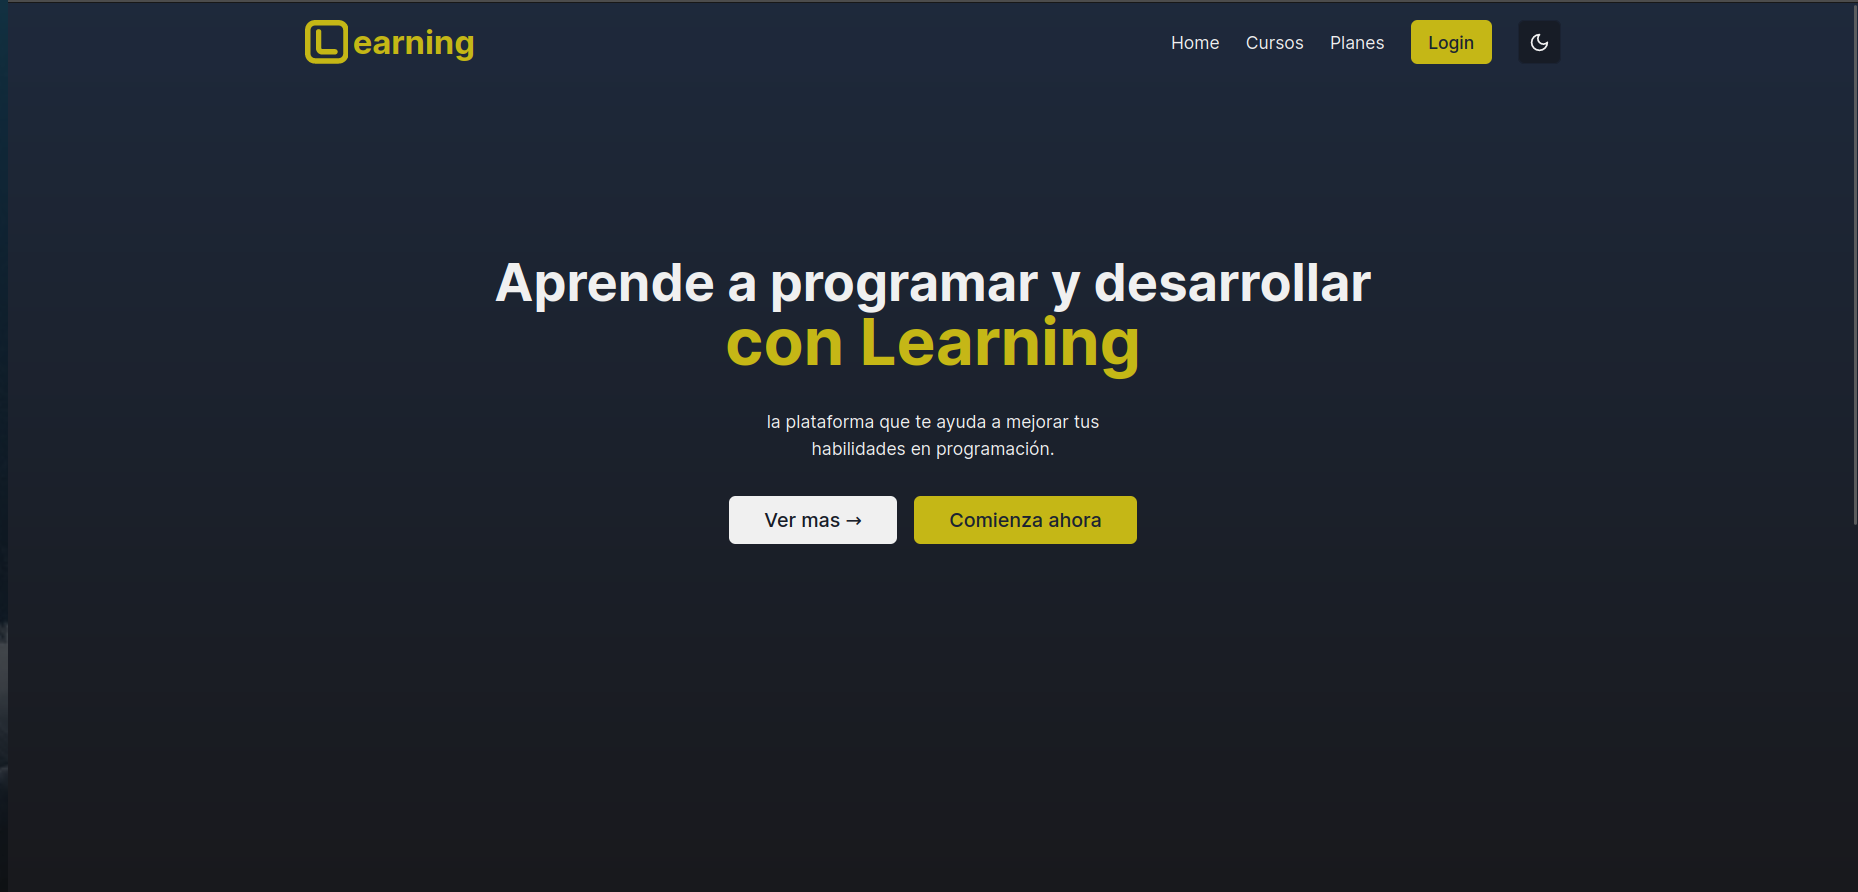
\includegraphics[width=1.0\textwidth]{img/H-DS.png}
    \caption{Home - Theme Dark and System}
  \end{figure}
  \begin{figure}[H]
    \centering
    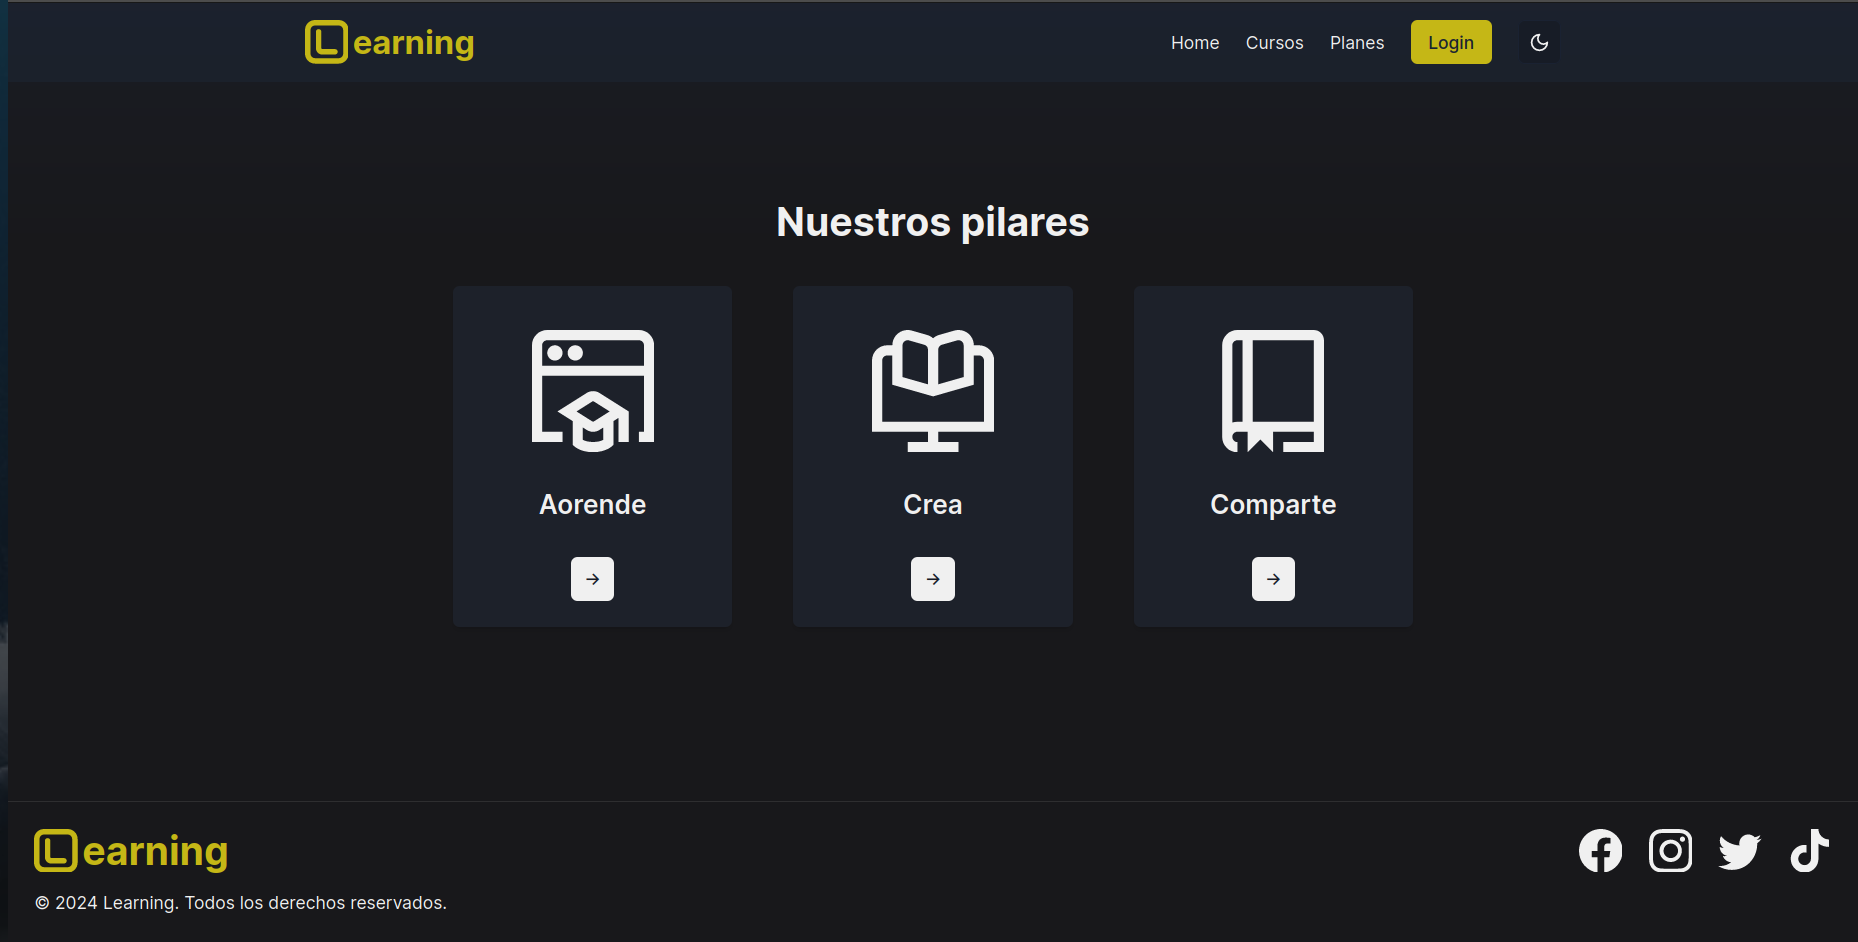
\includegraphics[width=1.0\textwidth]{img/H-DS2.png}
    \caption{Home - Theme Dark and System}
  \end{figure}
\subsection{Home - Theme Ligth}
  \begin{figure}[H]
    \centering
    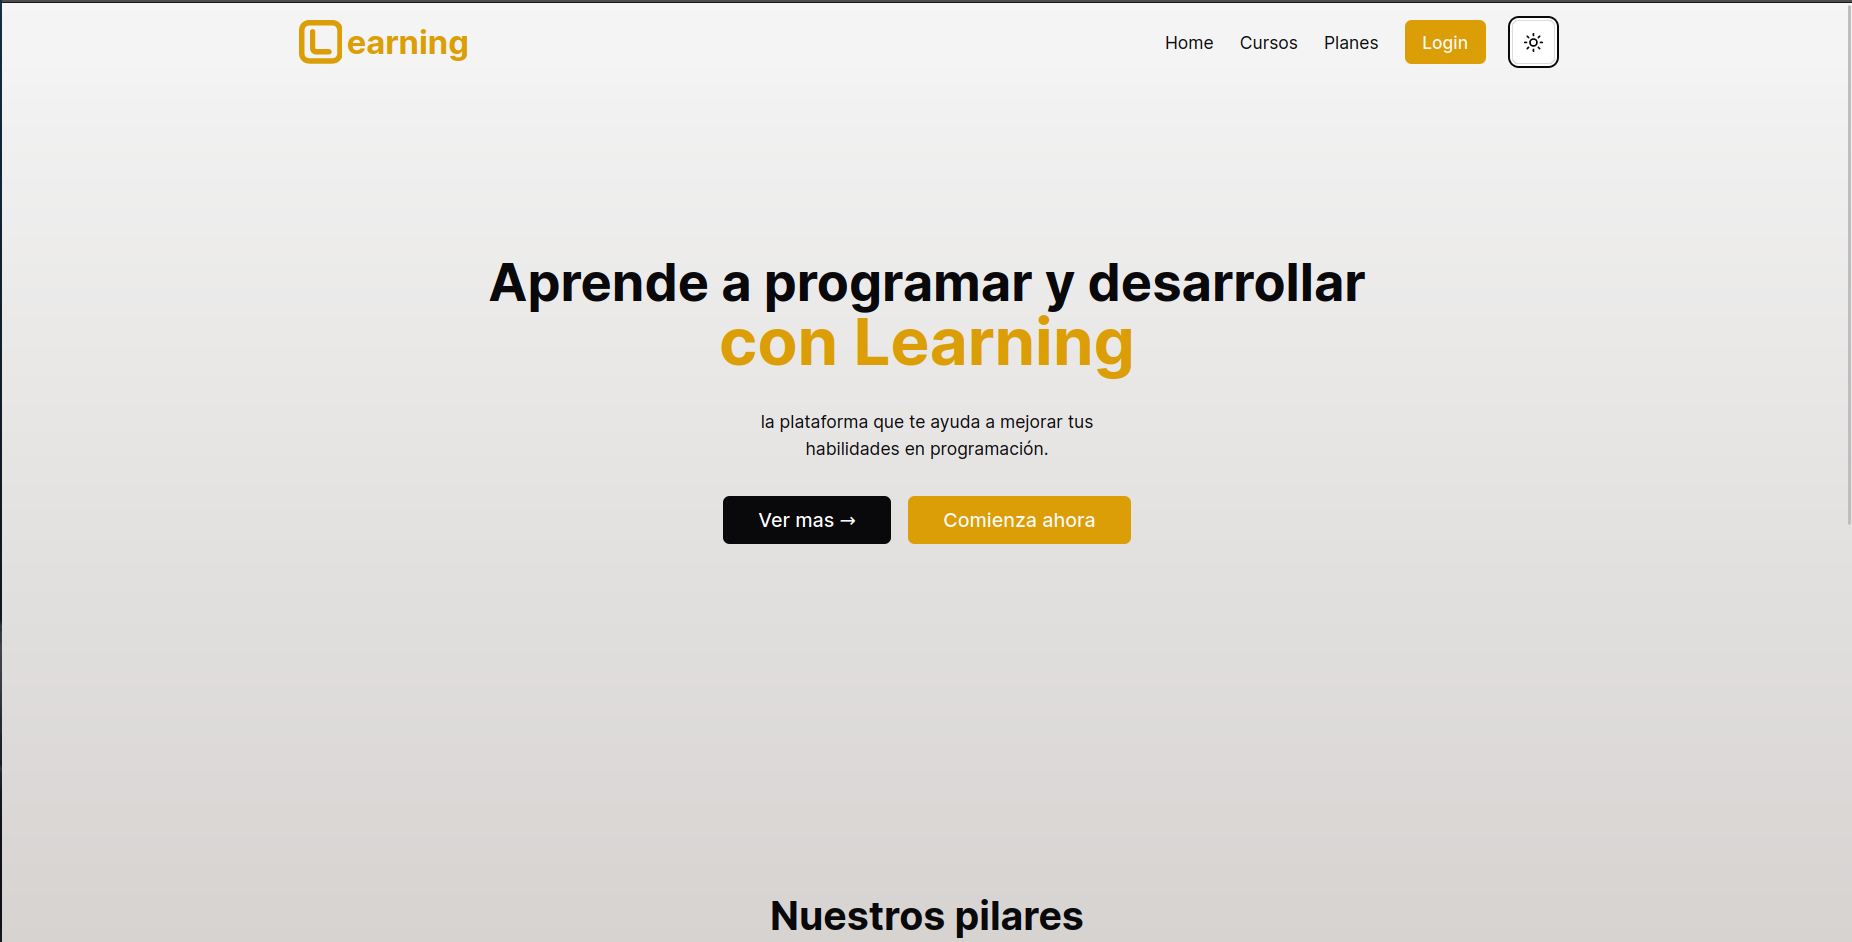
\includegraphics[width=1.0\textwidth]{img/H-L.png}
    \caption{Home - Theme Ligth}
  \end{figure}
  \begin{figure}[H]
    \centering
    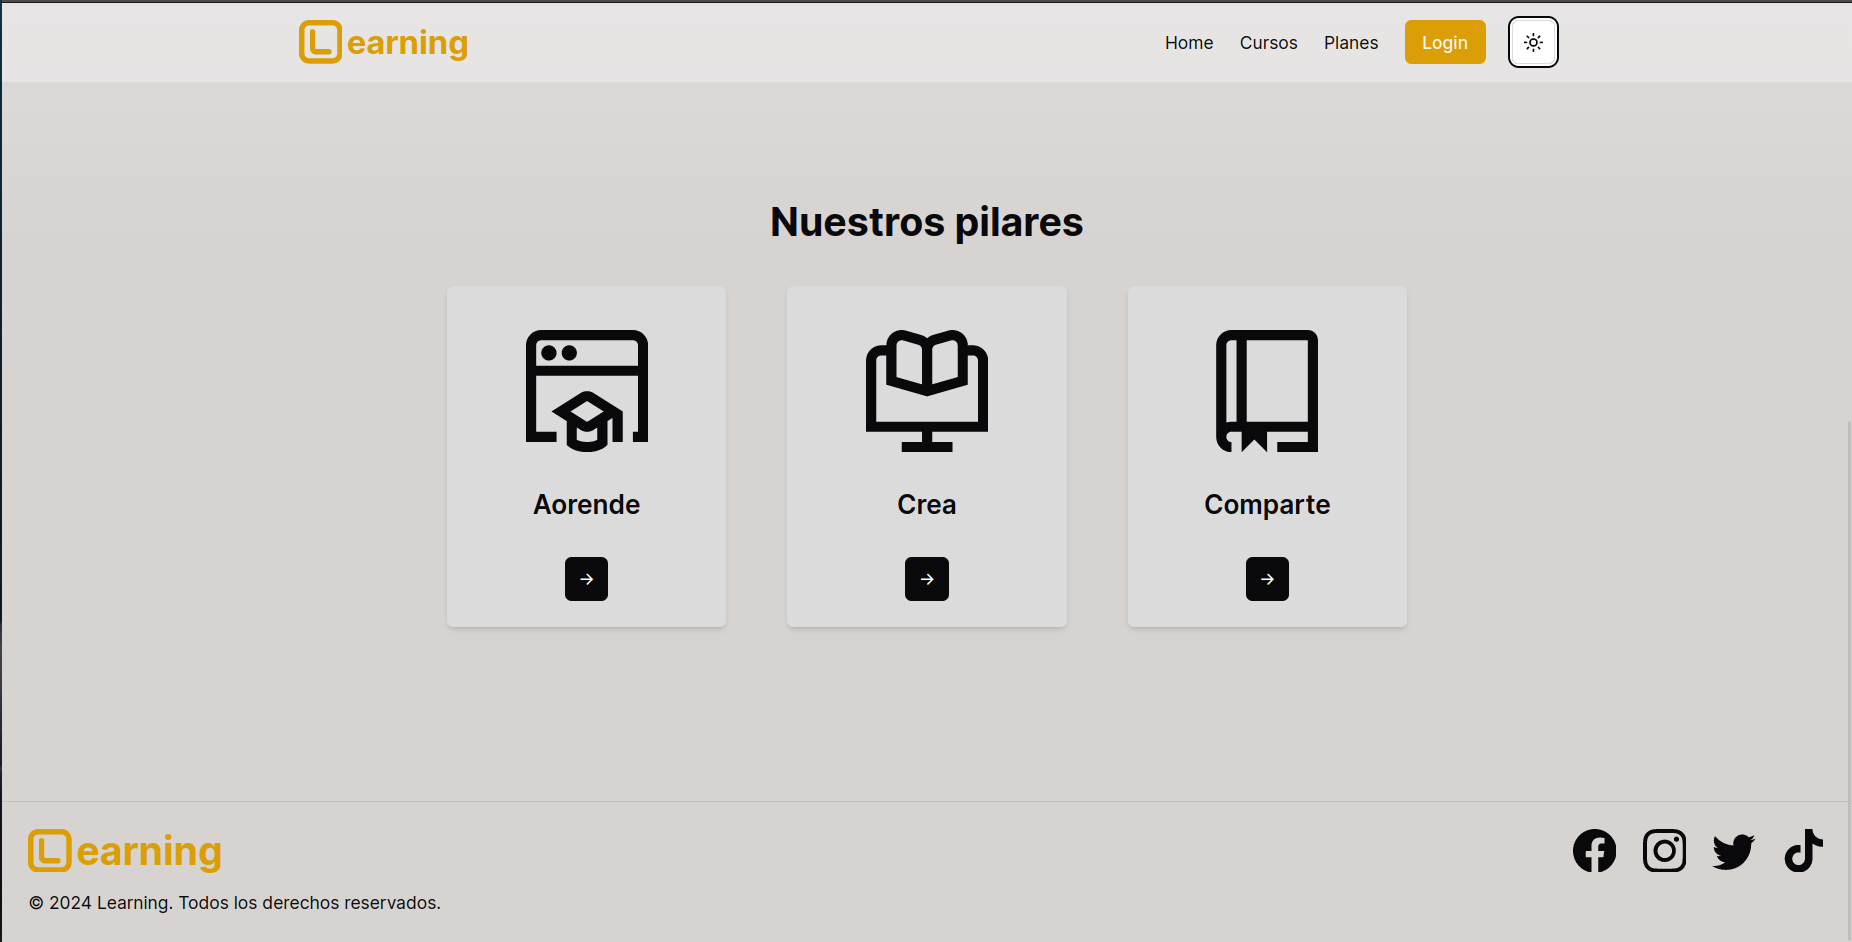
\includegraphics[width=1.0\textwidth]{img/H-L2.png}
    \caption{Home - Theme Ligth}
  \end{figure}
\subsection{Cursos - Theme Dark - System}
  \begin{figure}[H]
    \centering
    
\includegraphics[width=1.0\textwidth]{img/C-DS1.png}
    \caption{Cursos - Theme Dark and System}
  \end{figure}
  \begin{figure}[H]
    \centering
    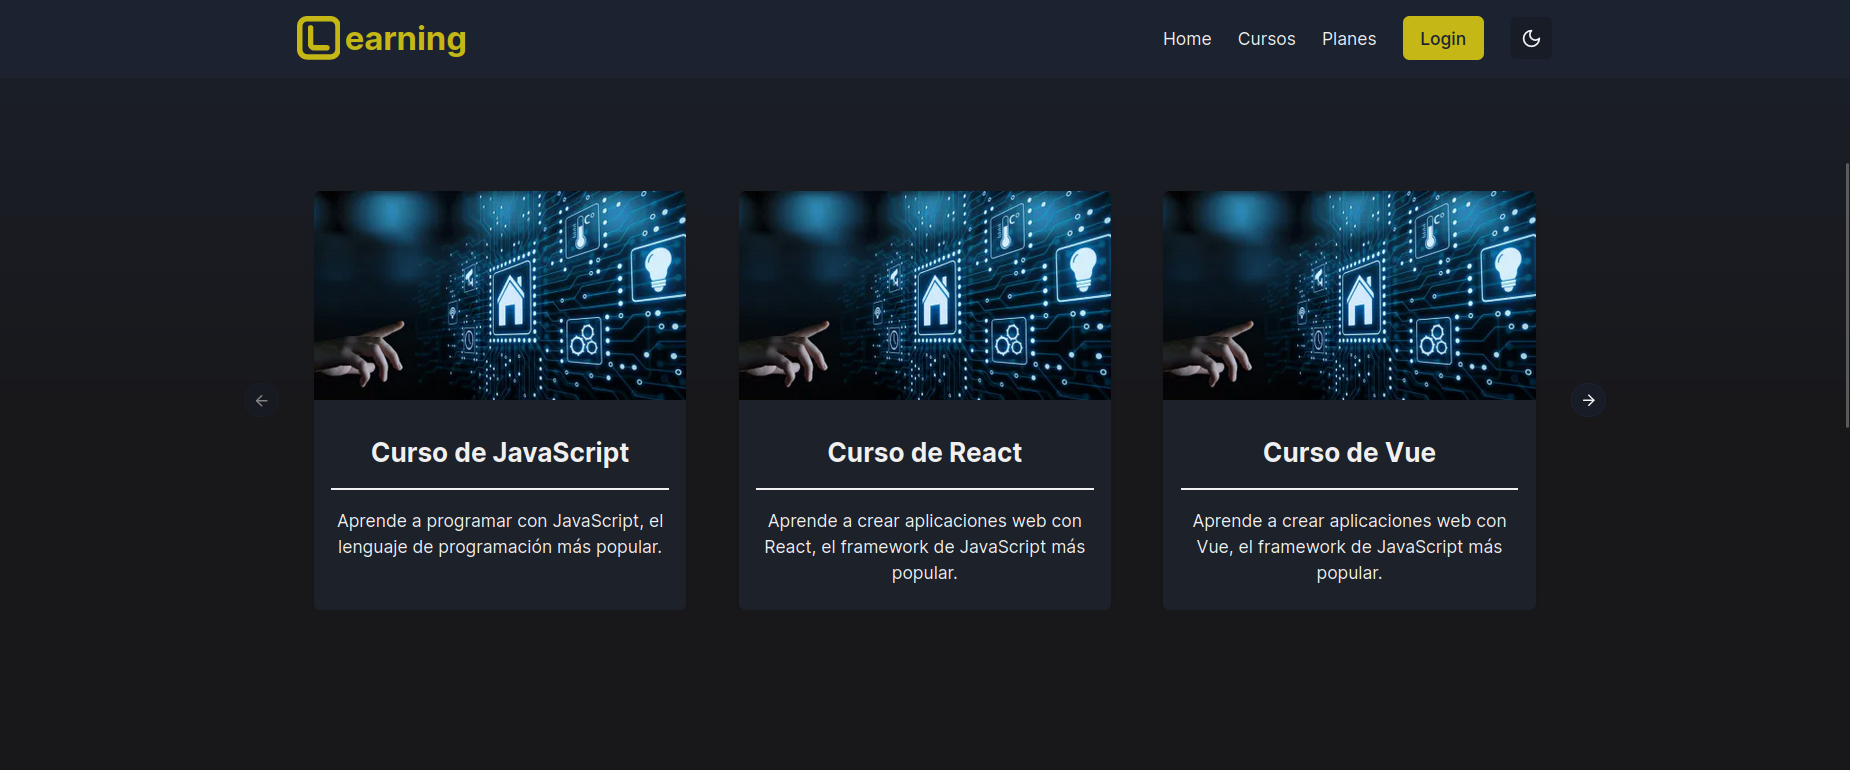
\includegraphics[width=1.0\textwidth]{img/C-DS2.png}
    \caption{Cursos - Theme Dark and System}
  \end{figure}
  \begin{figure}[H]
    \centering
    
\includegraphics[width=1.0\textwidth]{img/C-DS3.png}
    \caption{Cursos - Theme Dark and System}
  \end{figure}
  \begin{figure}[H]
    \centering
    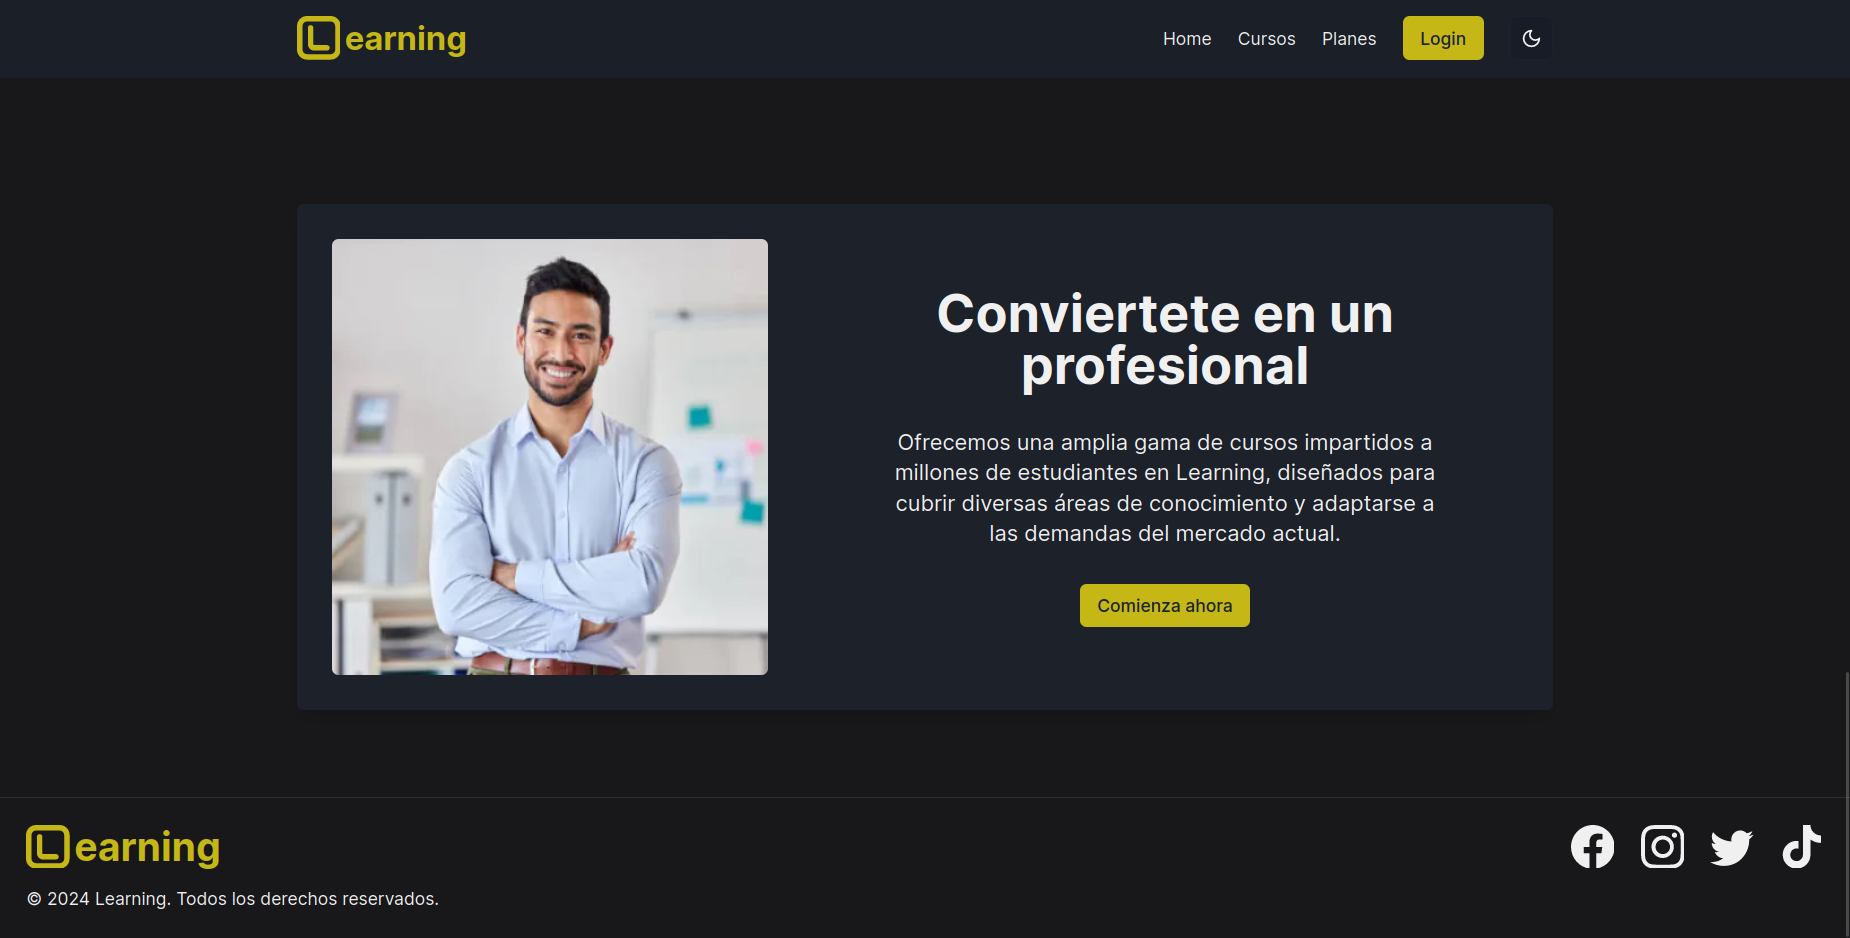
\includegraphics[width=1.0\textwidth]{img/C-DS4.png}
    \caption{Cursos - Theme Dark and System}
  \end{figure}
\subsection{Cursos - Theme Ligth}
  \begin{figure}[H]
    \centering
    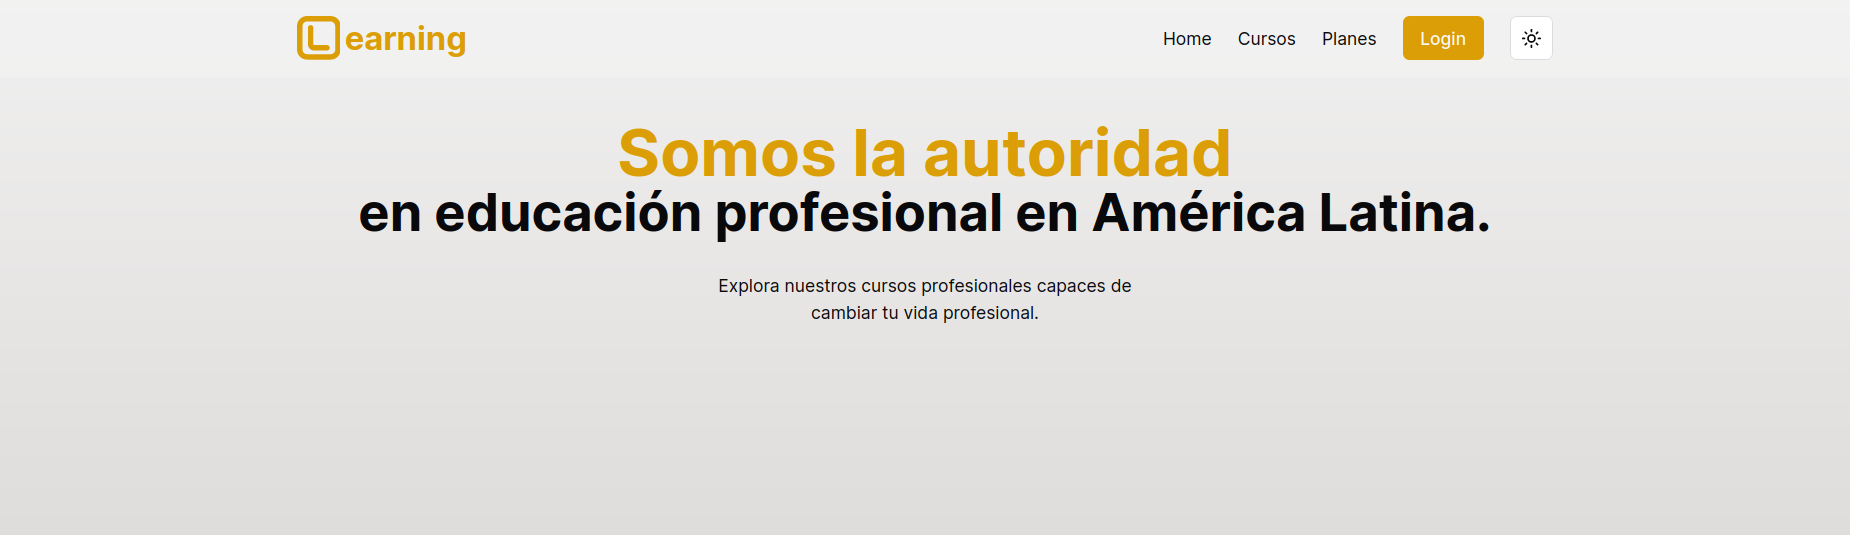
\includegraphics[width=1.0\textwidth]{img/C-L1.png}
    \caption{Cursos - Theme Ligth}
  \end{figure}
  \begin{figure}[H]
    \centering
    
\includegraphics[width=1.0\textwidth]{img/C-L2.png}
    \caption{Cursos - Theme Ligth}
  \end{figure}
  \begin{figure}[H]
    \centering
    
\includegraphics[width=1.0\textwidth]{img/C-L3.png}
    \caption{Cursos - Theme Ligth}
  \end{figure}
  \begin{figure}[H]
    \centering
    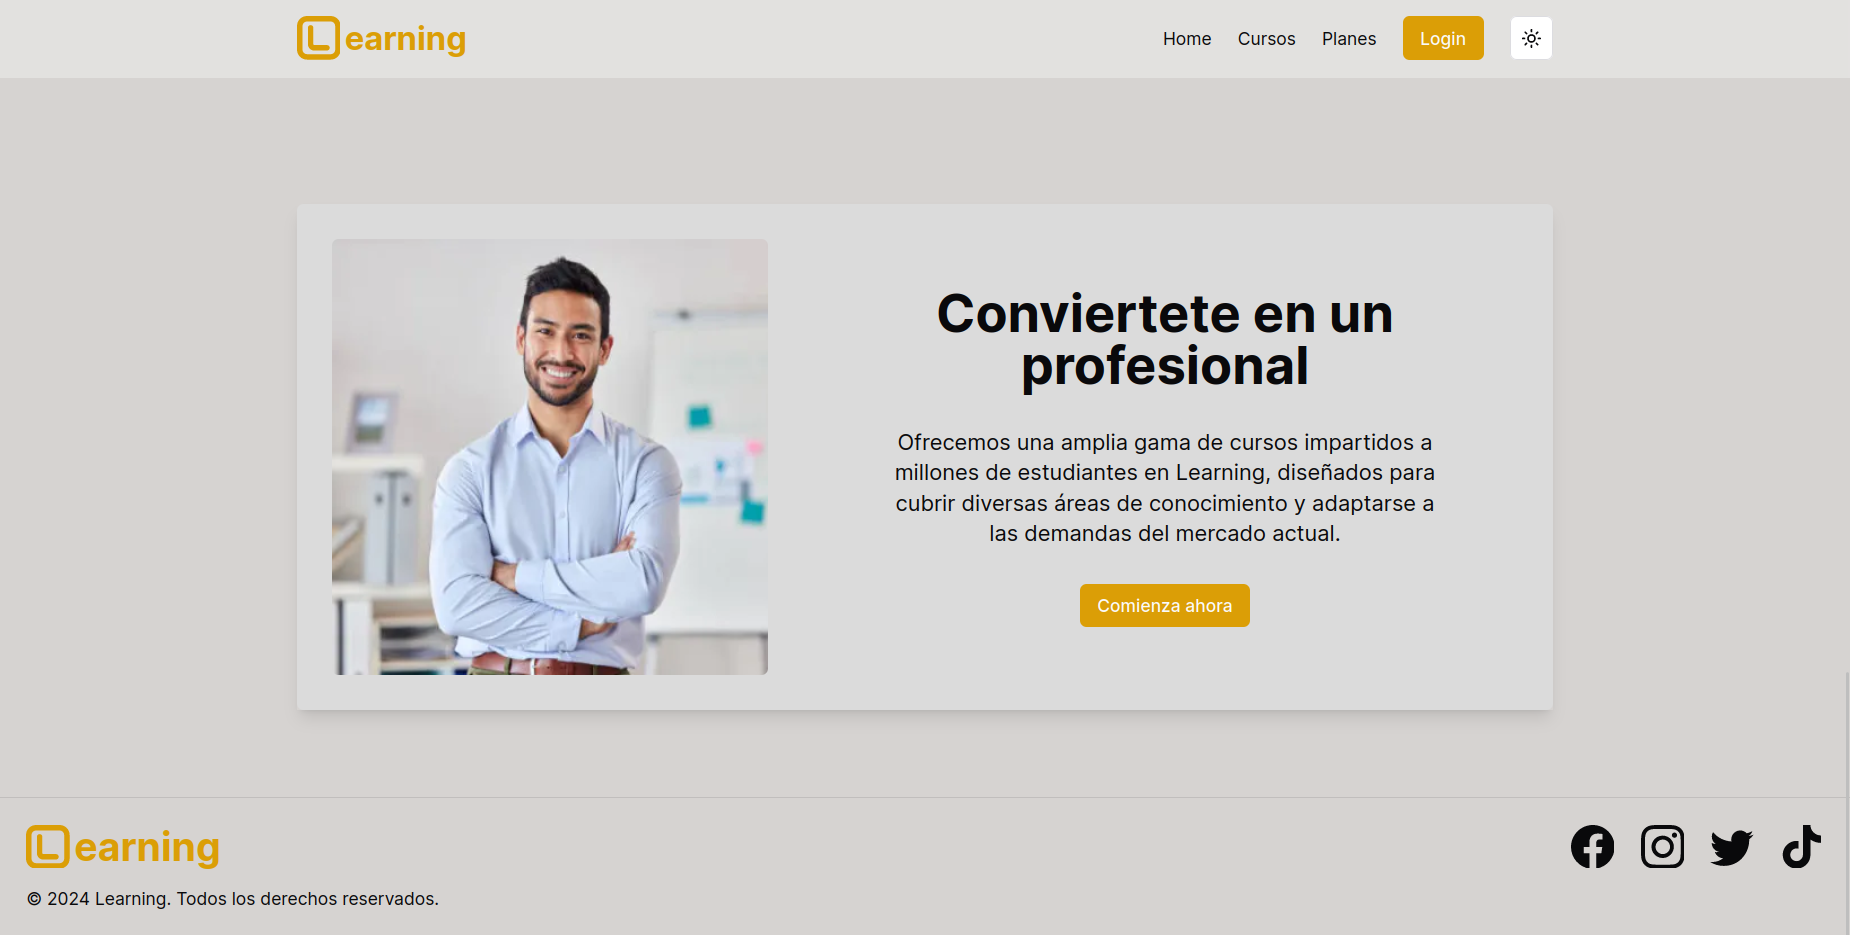
\includegraphics[width=1.0\textwidth]{img/C-L4.png}
    \caption{Cursos - Theme Ligth}
  \end{figure}










